\section{\label{simulations}Numerical simulations}

The simulations process were performed on a straight corridor of length $L=$ 28~m (with periodic boundary conditions) and variable width $w$. We explored widths ranging from $w=2$~m to $w=40$~m. The corridor had two side walls, placed at $y=0$ and $y=w$, respectively. The length of each wall was $L$. The pedestrians were modeled as soft spheres of radius $R_i=0.23$~m. This size was fixed according to Ref.~\cite{metric_handbook}. Initially, the individuals were randomly distributed along the corridor with a fixed global density (p/m$^{2}$) and with random initial velocities, resembling a Gaussian distribution with null mean value. We explored global density values in the range 1p~m$^{-2}$ $<\rho<$ 9 p~m$^{-2}$. We did not explore extreme densities (say $\rho>9$) because we exclude injuring situations. The number of pedestrians in the simulation was given by the global density and the corridor dimensions chosen in each case. \\

The simulations were supported by LAMMPS molecular dynamics simulator with parallel computing capabilities \cite{plimpton}.
The time integration algorithm followed the velocity Verlet scheme with a time step of $10^{-4}$~s. All the necessary parameters
were set to the same values as in previous works (see Refs. \cite{sticco,Dorso5}), except for the friction coefficient $\kappa$. In this work we use the common value $\kappa=2.4 \times 10^{5}$ Kg~m$^{-1}$~s$^{-1}$, but we eventually set the newly defined parameters $\kappa_i=2.4 \times 10^{6}$ Kg~m$^{-1}$~s$^{-1}$  and $\kappa_w=2.4 \times 10^{6}$ Kg~m$^{-1}$~s$^{-1}$, being $\kappa_i$ and $\kappa_w$ the pedestrian-pedestrian friction coefficient and the pedestrian-wall friction coefficient, respectively. \\

We implemented special modules in C++ for upgrading the LAMMPS capabilities to attain the social force model simulations. We also checked over the LAMMPS output with previous computations (see Refs. \cite{Dorso1, Dorso2,Dorso3, Dorso4,Dorso6}).\\

The desired velocity for each pedestrian $i$ was $\vec{v}_d^{~(i)}=1$~m/s~$\hat{e}_d^{~(i)}$, where the target $\hat{e}_d^{~(i)}$ was set as $\hat{e}_d^{~(i)}=(L,y_i)\left \| (L,y_i) \right \|^{-1}$, being $L$ the \textit{x}-location of the end at the corridor and $y_i$ the \textit{y}-location corresponding to the \textit{ith} pedestrian (see Fig.~\ref{pasillo}). This allowed the pedestrians to move from left to right in an unidirectional flow. Pedestrians that surpassed $x=L$ were re-injected at $x=0$, preserving their current velocity and \textit{y}-location (\textit{i.e.} periodic boundary conditions). This mechanism was carried out in order to keep
the crowd size unchanged.\\

The measurements were taken once the system reached the stationary state ($t=30$~s), while the configurations of the systems were recorded every 0.05~s, that is, at intervals as short as 10\% of the pedestrian’s relaxation time (see Sec. \ref{sfm}). The recorded magnitudes were the pedestrian’s positions and velocities for each process. We also computed the clusterering structures using a LAMMPS built in function.\\
  
We warn the reader that, for simplicity, we will not include the units corresponding to the numerical results. Remember that the friction coefficient has units $\left [ \kappa \right]=$Kg~m$^{-1}$~s$^{-1}$, the density $\left [ \rho \right]=$p~m$^{-2}$  and the flow  $\left [ J \right ]=$p~m$^{-1}$~s$^{-1}$.


\begin{figure}[htbp!]
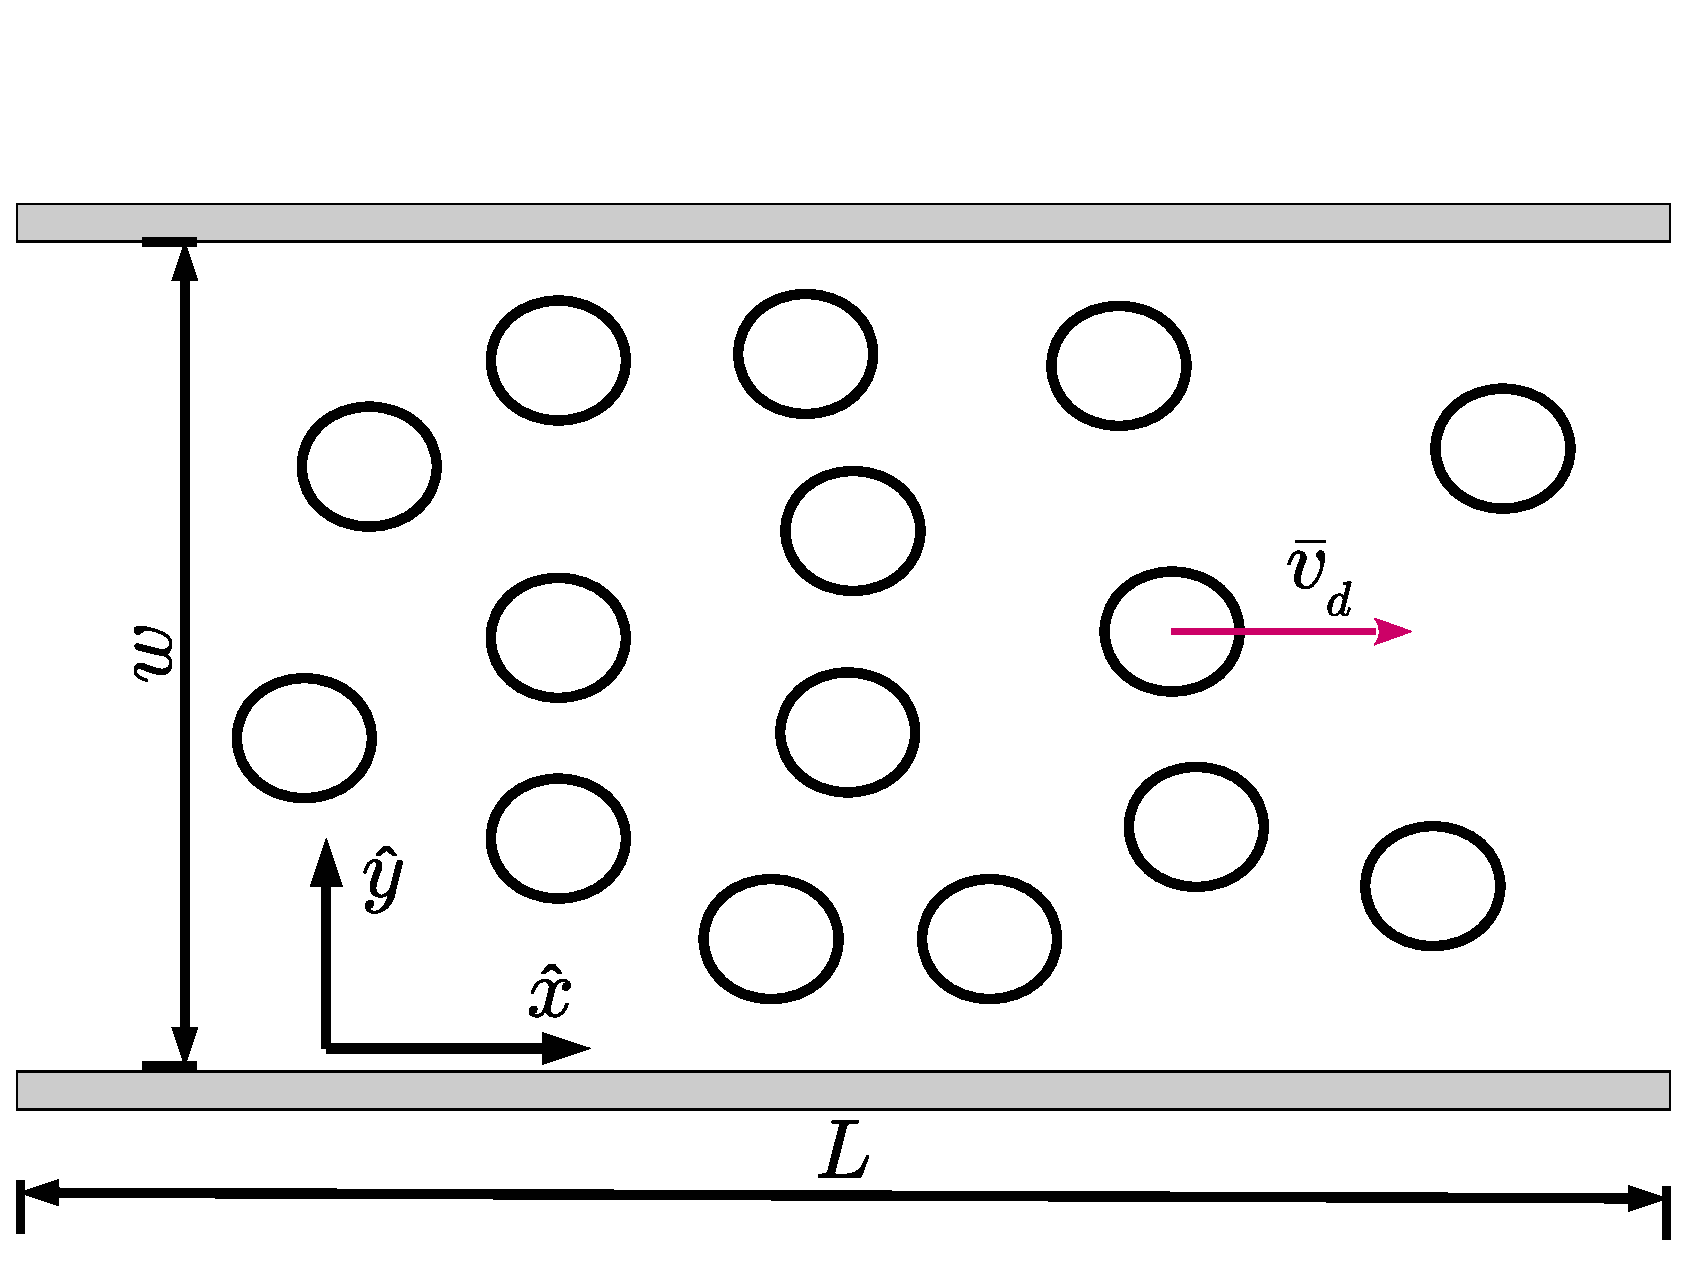
\includegraphics[width=\columnwidth]
{./plots/corridor.eps}
\caption{\label{corridor} Schematic diagram for individuals in the corridor. 
The circles represent pedestrians moving from left to right. $w$ represents the corridor width, $L$ represents the length. The rectangular boxes are upper and lower blocks that represent the walls of the corridor. The dashed circle in the middle corresponds to the measurement region.}
\end{figure}
